%  21 Nov 2024 15:30:16
\documentclass{article}
\usepackage{geometry,booktabs,longtable,pdflscape,rotating,threeparttable,subcaption,graphicx,float,}
\usepackage{tabularx,xcolor,colortbl,}
\usepackage{hyperref}
\hypersetup{                           colorlinks=true,                   linkcolor={blue!50!black},                    filecolor={blue!50!black},                 urlcolor={blue!80!black},                     }                              \date{}
\geometry{verbose,letterpaper,lmargin=2.5cm,tmargin=2.5cm}

\begin{document}

\title{Descriptives for Displacement Analysis Sample}
\maketitle
\section{Summary Table}
\begin{table}[p] \centering 
\begin{threeparttable} 
\caption{Sample Characteristics at Baseline (Quarter before Disp t=-1)}    
\begin{tabular}{l *{3}{c}} 
\toprule
                                                        & (1)                 &    (2)              &    (3)              \\
                                                        & Full Sample         &    Displaced        &    Non-Displaced    \\
                                                        &                     &    Workers          &    Workers          \\
\midrule
 \multicolumn{4}{l}{\textbf{Panel A: Demographics}} \\ 
Birth Year                                              &              1957.1 &              1956.8 &              1957.4 \\ 
                                                        &               [9.0] &               [8.9] &               [9.1] \\ 
Age                                                     &                41.6 &                41.8 &                41.3 \\ 
                                                        &               [8.2] &               [8.1] &               [8.2] \\ 
Female                                                  &                 0.3 &                 0.3 &                 0.3 \\ 
                                                        &               [0.5] &               [0.5] &               [0.5] \\ 
Years of Schooling                                      &                11.6 &                11.5 &                11.6 \\ 
                                                        &               [2.3] &               [2.3] &               [2.3] \\ 
 \multicolumn{4}{l}{\textbf{Panel B: Earnings Variables}} \\ 
Earnings                                                &             12111.7 &             12092.3 &             12131.1 \\ 
                                                        &            [3465.6] &            [3336.8] &            [3594.3] \\ 
Log Earnings                                            &                 9.4 &                 9.4 &                 9.4 \\ 
                                                        &               [0.3] &               [0.3] &               [0.3] \\ 
Employed                                                &                   1 &                   1 &                   1 \\ 
                                                        &                 [0] &                 [0] &                 [0] \\ 
 \multicolumn{4}{l}{\textbf{Panel C: Firm Characteristics}} \\ 
Firm size                                               &               498.8 &               505.2 &               492.4 \\ 
                                                        &             [432.2] &             [434.5] &             [430.3] \\ 
Cominbed firm effect (ind + size + rand)                &                0.02 &                0.02 &                0.02 \\ 
                                                        &              [0.08] &              [0.08] &              [0.08] \\ 
\addlinespace
Number of Spells                                        &                 724 &                 362 &                 362 \\
\bottomrule
\end{tabular}
\textbf{Notes:} Average characteristics of individuals.
Standard deviations in brackets. 
\end{threeparttable} 
\end{table}
\clearpage 
 
\begin{table}[htbp] 
\centering 
\begin{threeparttable} 
\caption{Summary Statistics by Displacement Status} 

\centering
\begin{tabular}{llll}
\toprule
\multicolumn{1}{c}{} &
  \multicolumn{1}{r}{All workers} &
  \multicolumn{1}{r}{Non-Displaced} &
  \multicolumn{1}{r}{Displaced} \\
\midrule
\multicolumn{1}{l}{Birth Year} &
  \multicolumn{1}{c}{1957.1} &
  \multicolumn{1}{c}{1957.1} &
  \multicolumn{1}{c}{1957.1} \\
\multicolumn{1}{l}{} &
  \multicolumn{1}{c}{[9.0]} &
  \multicolumn{1}{c}{[9.0]} &
  \multicolumn{1}{c}{[9.0]} \\
\multicolumn{1}{l}{Age} &
  \multicolumn{1}{c}{41.6} &
  \multicolumn{1}{c}{41.6} &
  \multicolumn{1}{c}{41.6} \\
\multicolumn{1}{l}{} &
  \multicolumn{1}{c}{[8.2]} &
  \multicolumn{1}{c}{[8.2]} &
  \multicolumn{1}{c}{[8.2]} \\
\multicolumn{1}{l}{Female} &
  \multicolumn{1}{c}{0.3} &
  \multicolumn{1}{c}{0.3} &
  \multicolumn{1}{c}{0.3} \\
\multicolumn{1}{l}{} &
  \multicolumn{1}{c}{[0.5]} &
  \multicolumn{1}{c}{[0.5]} &
  \multicolumn{1}{c}{[0.5]} \\
\multicolumn{1}{l}{Years of Schooling} &
  \multicolumn{1}{c}{11.6} &
  \multicolumn{1}{c}{11.6} &
  \multicolumn{1}{c}{11.6} \\
\multicolumn{1}{l}{} &
  \multicolumn{1}{c}{[2.3]} &
  \multicolumn{1}{c}{[2.3]} &
  \multicolumn{1}{c}{[2.3]} \\
\multicolumn{1}{l}{Earnings} &
  \multicolumn{1}{c}{12111.7} &
  \multicolumn{1}{c}{12111.7} &
  \multicolumn{1}{c}{12111.7} \\
\multicolumn{1}{l}{} &
  \multicolumn{1}{c}{[3465.6]} &
  \multicolumn{1}{c}{[3465.6]} &
  \multicolumn{1}{c}{[3465.6]} \\
\multicolumn{1}{l}{Log Earnings} &
  \multicolumn{1}{c}{9.4} &
  \multicolumn{1}{c}{9.4} &
  \multicolumn{1}{c}{9.4} \\
\multicolumn{1}{l}{} &
  \multicolumn{1}{c}{[0.3]} &
  \multicolumn{1}{c}{[0.3]} &
  \multicolumn{1}{c}{[0.3]} \\
\multicolumn{1}{l}{Employed} &
  \multicolumn{1}{c}{1.0} &
  \multicolumn{1}{c}{1.0} &
  \multicolumn{1}{c}{1.0} \\
\multicolumn{1}{l}{} &
  \multicolumn{1}{c}{[0.0]} &
  \multicolumn{1}{c}{[0.0]} &
  \multicolumn{1}{c}{[0.0]} \\
\multicolumn{1}{l}{Firm size} &
  \multicolumn{1}{c}{498.8} &
  \multicolumn{1}{c}{498.8} &
  \multicolumn{1}{c}{498.8} \\
\multicolumn{1}{l}{} &
  \multicolumn{1}{c}{[432.2]} &
  \multicolumn{1}{c}{[432.2]} &
  \multicolumn{1}{c}{[432.2]} \\
\multicolumn{1}{l}{Cominbed firm effect (ind + size + rand)} &
  \multicolumn{1}{c}{0.0} &
  \multicolumn{1}{c}{0.0} &
  \multicolumn{1}{c}{0.0} \\
\multicolumn{1}{l}{} &
  \multicolumn{1}{c}{[0.1]} &
  \multicolumn{1}{c}{[0.1]} &
  \multicolumn{1}{c}{[0.1]} \\
\midrule
\multicolumn{1}{l}{Number of Observations} &
  \multicolumn{1}{c}{724} &
  \multicolumn{1}{c}{724} &
  \multicolumn{1}{c}{724} \\
\multicolumn{1}{l}{Number of Establishments} &
  \multicolumn{1}{c}{94} &
  \multicolumn{1}{c}{92} &
  \multicolumn{1}{c}{93} \\
\bottomrule
\end{tabular}

 \footnotesize  
\textbf{Notes:} Average characteristics of individuals. Standard deviations in brackets. 
\end{threeparttable} 
\end{table}
\begin{table}[htbp] 
\centering 
\begin{threeparttable} 
\caption{Summary Statistics with Percentiles} 

\centering
\begin{tabular}{lllllllll}
\toprule
\multicolumn{1}{c}{} &
  \multicolumn{1}{c}{10th pct} &
  \multicolumn{1}{c}{25th pct} &
  \multicolumn{1}{c}{50th pct} &
  \multicolumn{1}{c}{75th pct} &
  \multicolumn{1}{c}{90th pct} &
  \multicolumn{1}{c}{Mean} &
  \multicolumn{1}{c}{SD} &
  \multicolumn{1}{c}{N} \\
\midrule
\multicolumn{1}{l}{Birth Year} &
  \multicolumn{1}{c}{1945.00} &
  \multicolumn{1}{c}{1950.00} &
  \multicolumn{1}{c}{1957.00} &
  \multicolumn{1}{c}{1964.00} &
  \multicolumn{1}{c}{1969.00} &
  \multicolumn{1}{c}{1957.08} &
  \multicolumn{1}{c}{[9.02]} &
  \multicolumn{1}{c}{724} \\
\multicolumn{1}{l}{Age} &
  \multicolumn{1}{c}{30.00} &
  \multicolumn{1}{c}{35.00} &
  \multicolumn{1}{c}{41.00} &
  \multicolumn{1}{c}{49.00} &
  \multicolumn{1}{c}{53.00} &
  \multicolumn{1}{c}{41.55} &
  \multicolumn{1}{c}{[8.18]} &
  \multicolumn{1}{c}{724} \\
\multicolumn{1}{l}{Female} &
  \multicolumn{1}{c}{0.00} &
  \multicolumn{1}{c}{0.00} &
  \multicolumn{1}{c}{0.00} &
  \multicolumn{1}{c}{1.00} &
  \multicolumn{1}{c}{1.00} &
  \multicolumn{1}{c}{0.33} &
  \multicolumn{1}{c}{[0.47]} &
  \multicolumn{1}{c}{724} \\
\multicolumn{1}{l}{Years of Schooling} &
  \multicolumn{1}{c}{8.00} &
  \multicolumn{1}{c}{10.00} &
  \multicolumn{1}{c}{11.00} &
  \multicolumn{1}{c}{14.00} &
  \multicolumn{1}{c}{15.00} &
  \multicolumn{1}{c}{11.57} &
  \multicolumn{1}{c}{[2.35]} &
  \multicolumn{1}{c}{724} \\
\multicolumn{1}{l}{Earnings} &
  \multicolumn{1}{c}{8153.01} &
  \multicolumn{1}{c}{9516.40} &
  \multicolumn{1}{c}{11477.73} &
  \multicolumn{1}{c}{14079.55} &
  \multicolumn{1}{c}{16955.90} &
  \multicolumn{1}{c}{12111.68} &
  \multicolumn{1}{c}{[3465.57]} &
  \multicolumn{1}{c}{724} \\
\multicolumn{1}{l}{Log Earnings} &
  \multicolumn{1}{c}{9.01} &
  \multicolumn{1}{c}{9.16} &
  \multicolumn{1}{c}{9.35} &
  \multicolumn{1}{c}{9.55} &
  \multicolumn{1}{c}{9.74} &
  \multicolumn{1}{c}{9.36} &
  \multicolumn{1}{c}{[0.28]} &
  \multicolumn{1}{c}{724} \\
\multicolumn{1}{l}{Employed} &
  \multicolumn{1}{c}{1.00} &
  \multicolumn{1}{c}{1.00} &
  \multicolumn{1}{c}{1.00} &
  \multicolumn{1}{c}{1.00} &
  \multicolumn{1}{c}{1.00} &
  \multicolumn{1}{c}{1.00} &
  \multicolumn{1}{c}{[0.00]} &
  \multicolumn{1}{c}{724} \\
\multicolumn{1}{l}{Firm size} &
  \multicolumn{1}{c}{111.03} &
  \multicolumn{1}{c}{175.44} &
  \multicolumn{1}{c}{366.99} &
  \multicolumn{1}{c}{629.32} &
  \multicolumn{1}{c}{1099.06} &
  \multicolumn{1}{c}{498.81} &
  \multicolumn{1}{c}{[432.17]} &
  \multicolumn{1}{c}{724} \\
\multicolumn{1}{l}{Cominbed firm effect (ind + size + rand)} &
  \multicolumn{1}{c}{-0.14} &
  \multicolumn{1}{c}{0.04} &
  \multicolumn{1}{c}{0.06} &
  \multicolumn{1}{c}{0.06} &
  \multicolumn{1}{c}{0.07} &
  \multicolumn{1}{c}{0.02} &
  \multicolumn{1}{c}{[0.08]} &
  \multicolumn{1}{c}{724} \\
\bottomrule
\end{tabular}

\end{threeparttable} 
\end{table}
\begin{table}[htbp] 
\centering 
\begin{threeparttable} 
\caption{Industry Distribution by Displacement Status} 

\centering
\begin{tabular}{lll}
\toprule
\multicolumn{1}{c}{} &
  \multicolumn{1}{c}{Non-displaced} &
  \multicolumn{1}{c}{Displaced} \\
\midrule
\multicolumn{1}{c}{Mining} &
  \multicolumn{1}{c}{14.1} &
  \multicolumn{1}{c}{14.1} \\
\multicolumn{1}{c}{Construction} &
  \multicolumn{1}{c}{13.3} &
  \multicolumn{1}{c}{13.3} \\
\multicolumn{1}{c}{Manufacturing} &
  \multicolumn{1}{c}{13.8} &
  \multicolumn{1}{c}{13.8} \\
\multicolumn{1}{c}{Health} &
  \multicolumn{1}{c}{11.3} &
  \multicolumn{1}{c}{11.3} \\
\multicolumn{1}{c}{Finance} &
  \multicolumn{1}{c}{18.5} &
  \multicolumn{1}{c}{18.5} \\
\multicolumn{1}{c}{FCSL} &
  \multicolumn{1}{c}{18.5} &
  \multicolumn{1}{c}{18.5} \\
\multicolumn{1}{c}{Professional Services} &
  \multicolumn{1}{c}{10.5} &
  \multicolumn{1}{c}{10.5} \\
\multicolumn{1}{c}{Total} &
  \multicolumn{1}{c}{100.0} &
  \multicolumn{1}{c}{100.0} \\
\bottomrule
\end{tabular}

\end{threeparttable} 
\end{table}
\begin{table}[htbp] 
\centering 
\begin{threeparttable} 
\caption{Number of Workers by Industry and Year} 

\centering
\begin{tabular}{llllllllllll}
\toprule
\multicolumn{1}{c}{} &
  \multicolumn{1}{r}{1993} &
  \multicolumn{1}{r}{1994} &
  \multicolumn{1}{r}{1995} &
  \multicolumn{1}{r}{1996} &
  \multicolumn{1}{r}{1997} &
  \multicolumn{1}{r}{1999} &
  \multicolumn{1}{r}{2000} &
  \multicolumn{1}{r}{2001} &
  \multicolumn{1}{r}{2002} &
  \multicolumn{1}{r}{2003} &
  \multicolumn{1}{r}{2004} \\
\midrule
\multicolumn{1}{l}{Mining} &
  \multicolumn{1}{r}{6} &
  \multicolumn{1}{r}{2} &
  \multicolumn{1}{r}{18} &
  \multicolumn{1}{r}{6} &
  \multicolumn{1}{r}{12} &
  \multicolumn{1}{r}{6} &
  \multicolumn{1}{r}{10} &
  \multicolumn{1}{r}{10} &
  \multicolumn{1}{r}{12} &
  \multicolumn{1}{r}{16} &
  \multicolumn{1}{r}{4} \\
\multicolumn{1}{l}{Construction} &
  \multicolumn{1}{r}{12} &
  \multicolumn{1}{r}{16} &
  \multicolumn{1}{r}{8} &
  \multicolumn{1}{r}{8} &
  \multicolumn{1}{r}{4} &
  \multicolumn{1}{r}{} &
  \multicolumn{1}{r}{14} &
  \multicolumn{1}{r}{12} &
  \multicolumn{1}{r}{12} &
  \multicolumn{1}{r}{6} &
  \multicolumn{1}{r}{4} \\
\multicolumn{1}{l}{Manufacturing} &
  \multicolumn{1}{r}{16} &
  \multicolumn{1}{r}{4} &
  \multicolumn{1}{r}{20} &
  \multicolumn{1}{r}{4} &
  \multicolumn{1}{r}{6} &
  \multicolumn{1}{r}{} &
  \multicolumn{1}{r}{18} &
  \multicolumn{1}{r}{6} &
  \multicolumn{1}{r}{8} &
  \multicolumn{1}{r}{8} &
  \multicolumn{1}{r}{10} \\
\multicolumn{1}{l}{Health} &
  \multicolumn{1}{r}{14} &
  \multicolumn{1}{r}{} &
  \multicolumn{1}{r}{14} &
  \multicolumn{1}{r}{2} &
  \multicolumn{1}{r}{10} &
  \multicolumn{1}{r}{4} &
  \multicolumn{1}{r}{6} &
  \multicolumn{1}{r}{18} &
  \multicolumn{1}{r}{4} &
  \multicolumn{1}{r}{6} &
  \multicolumn{1}{r}{4} \\
\multicolumn{1}{l}{Finance} &
  \multicolumn{1}{r}{12} &
  \multicolumn{1}{r}{14} &
  \multicolumn{1}{r}{24} &
  \multicolumn{1}{r}{} &
  \multicolumn{1}{r}{12} &
  \multicolumn{1}{r}{4} &
  \multicolumn{1}{r}{10} &
  \multicolumn{1}{r}{14} &
  \multicolumn{1}{r}{16} &
  \multicolumn{1}{r}{20} &
  \multicolumn{1}{r}{8} \\
\multicolumn{1}{l}{FCSL} &
  \multicolumn{1}{r}{10} &
  \multicolumn{1}{r}{10} &
  \multicolumn{1}{r}{14} &
  \multicolumn{1}{r}{12} &
  \multicolumn{1}{r}{6} &
  \multicolumn{1}{r}{} &
  \multicolumn{1}{r}{16} &
  \multicolumn{1}{r}{12} &
  \multicolumn{1}{r}{30} &
  \multicolumn{1}{r}{16} &
  \multicolumn{1}{r}{8} \\
\multicolumn{1}{l}{Professional Services} &
  \multicolumn{1}{r}{8} &
  \multicolumn{1}{r}{6} &
  \multicolumn{1}{r}{} &
  \multicolumn{1}{r}{8} &
  \multicolumn{1}{r}{6} &
  \multicolumn{1}{r}{10} &
  \multicolumn{1}{r}{} &
  \multicolumn{1}{r}{10} &
  \multicolumn{1}{r}{} &
  \multicolumn{1}{r}{16} &
  \multicolumn{1}{r}{12} \\
\bottomrule
\end{tabular}

 \footnotesize  
\textbf{Notes:} Each cell shows number of workers per cell 
\end{threeparttable} 
\end{table}
\section{Consistency Checks}
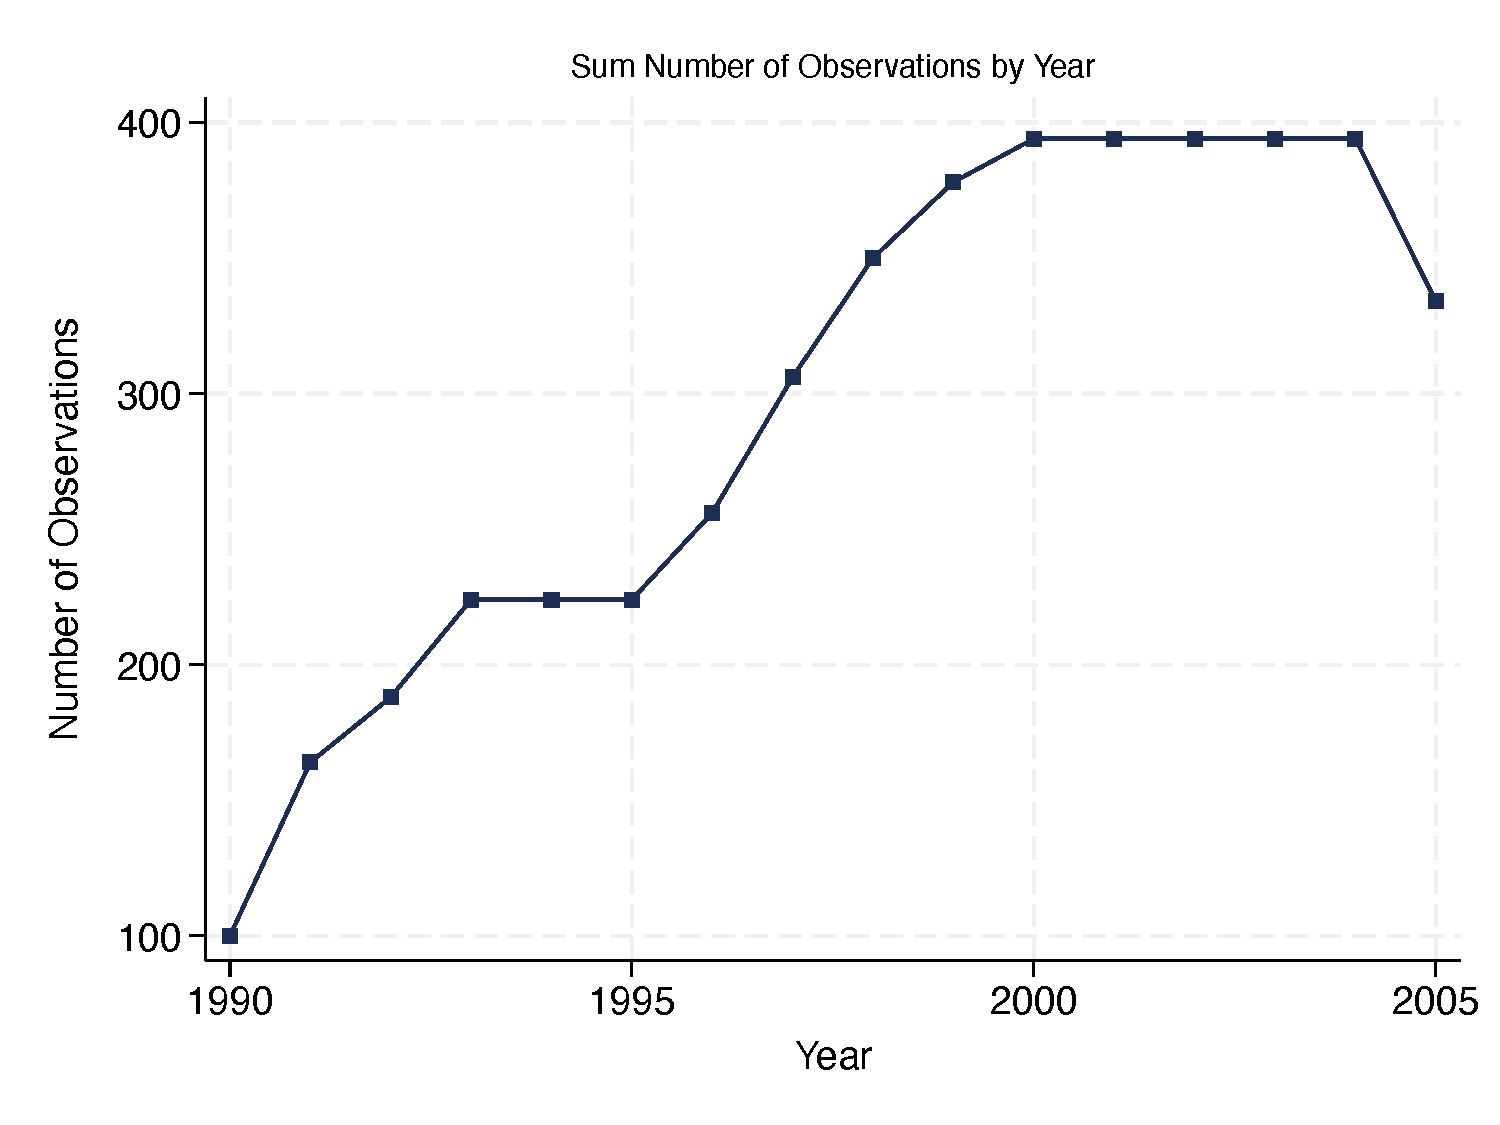
\includegraphics[width = .9\textwidth]{Consistency/counts_by_time.pdf} \\ 
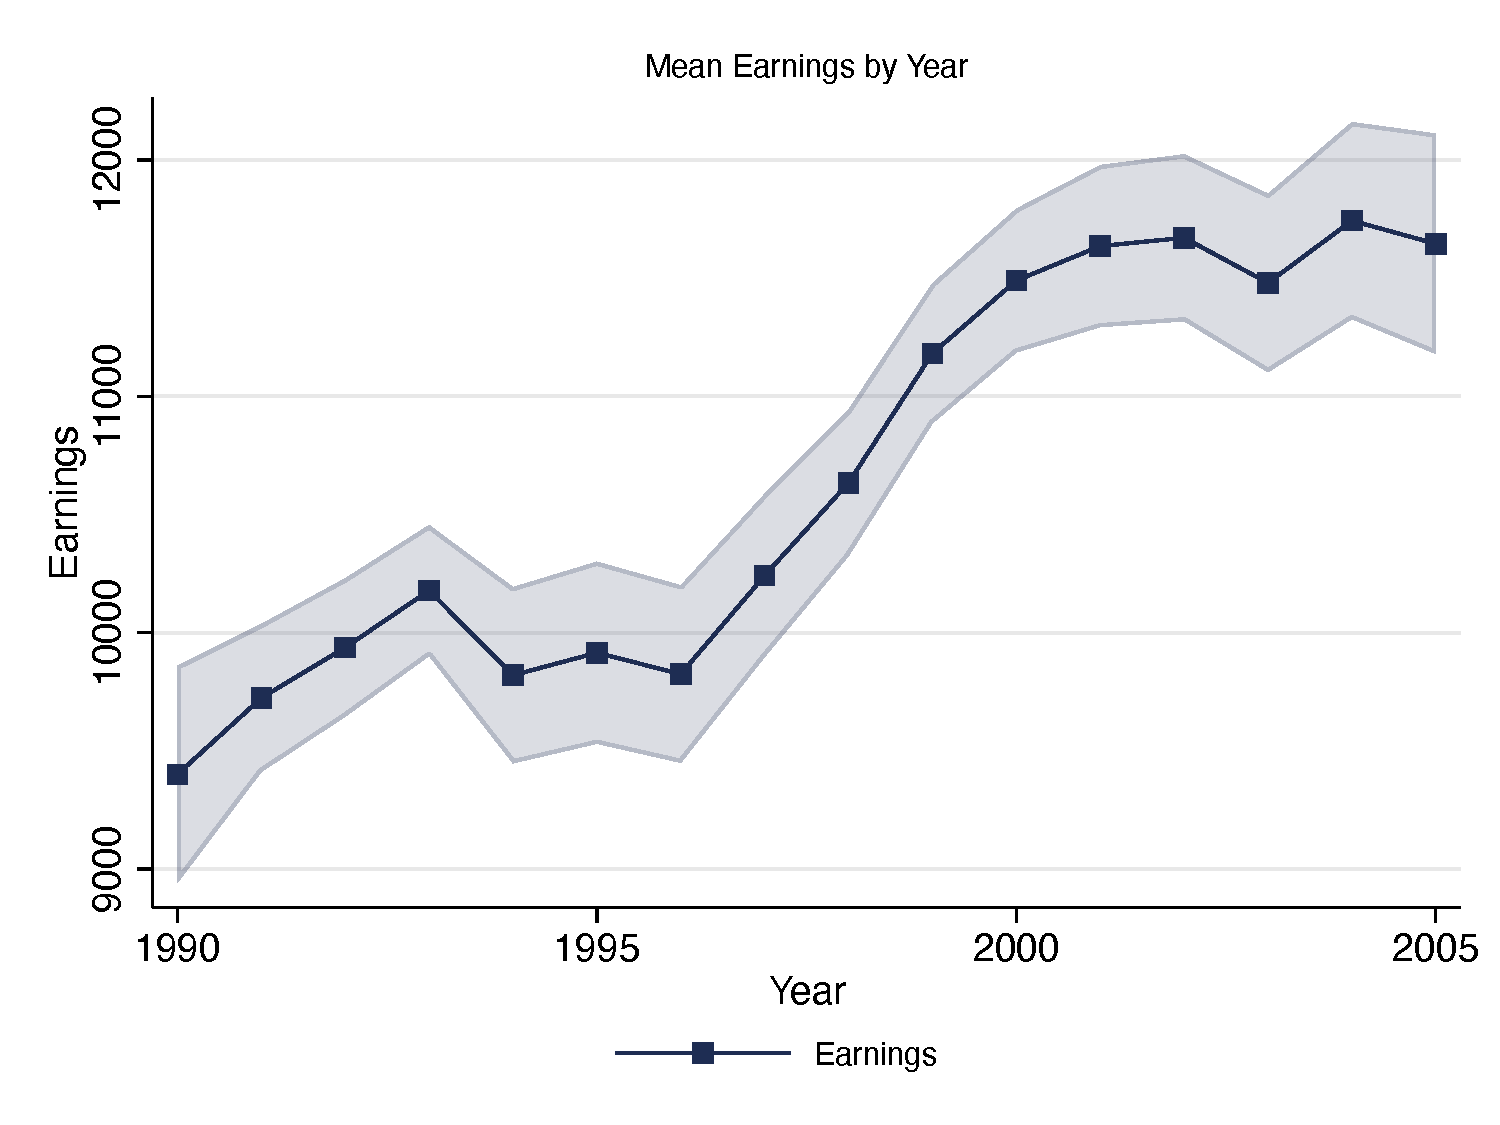
\includegraphics[width = .9\textwidth]{Consistency/earn_by_time.pdf} \\ 
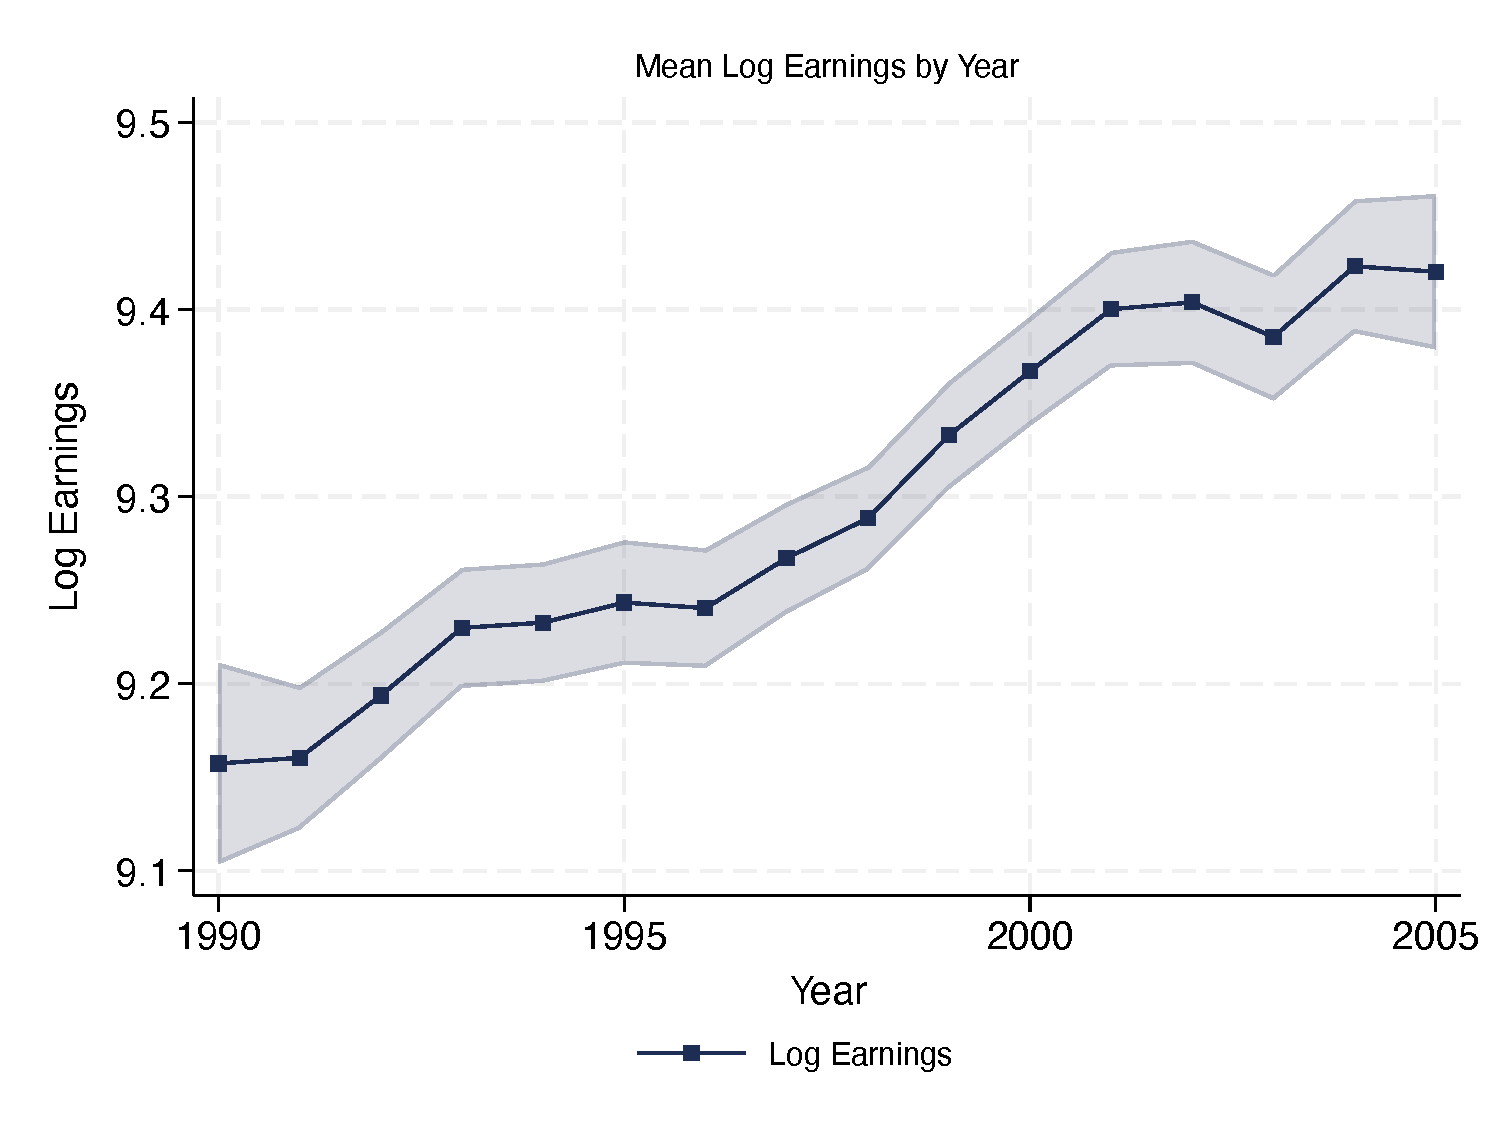
\includegraphics[width = .9\textwidth]{Consistency/logearn_by_time.pdf} \\ 
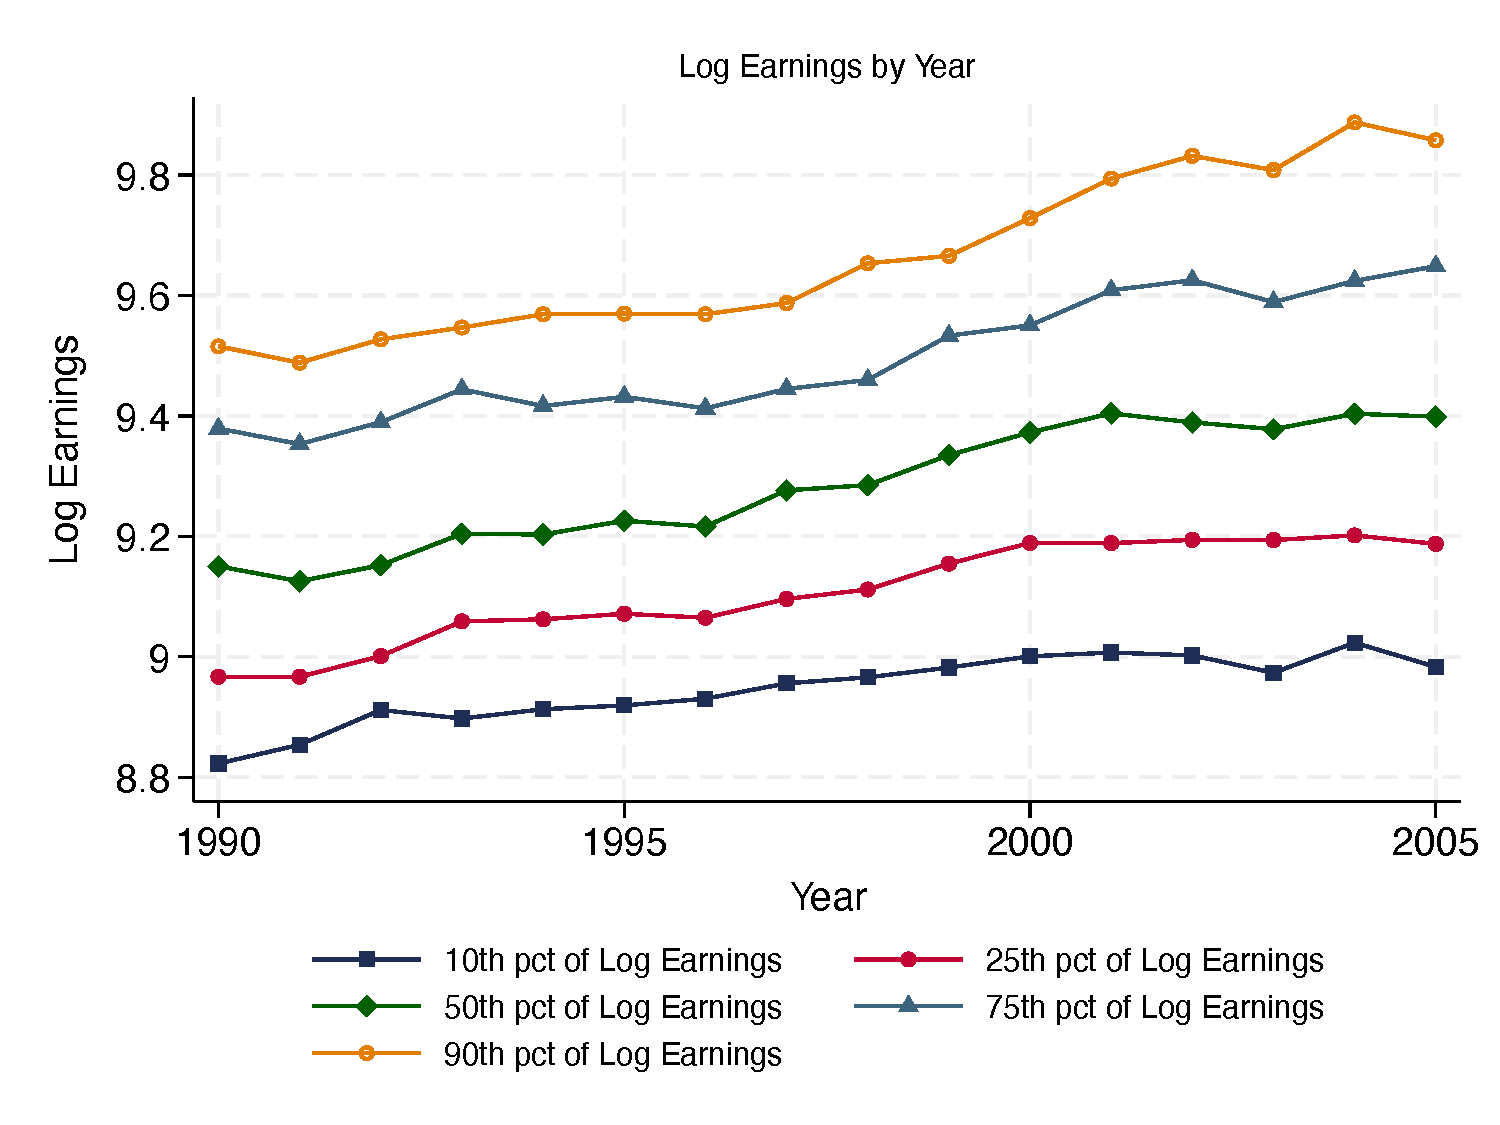
\includegraphics[width = .9\textwidth]{Consistency/logearn_by_year_pct.pdf} \\ 
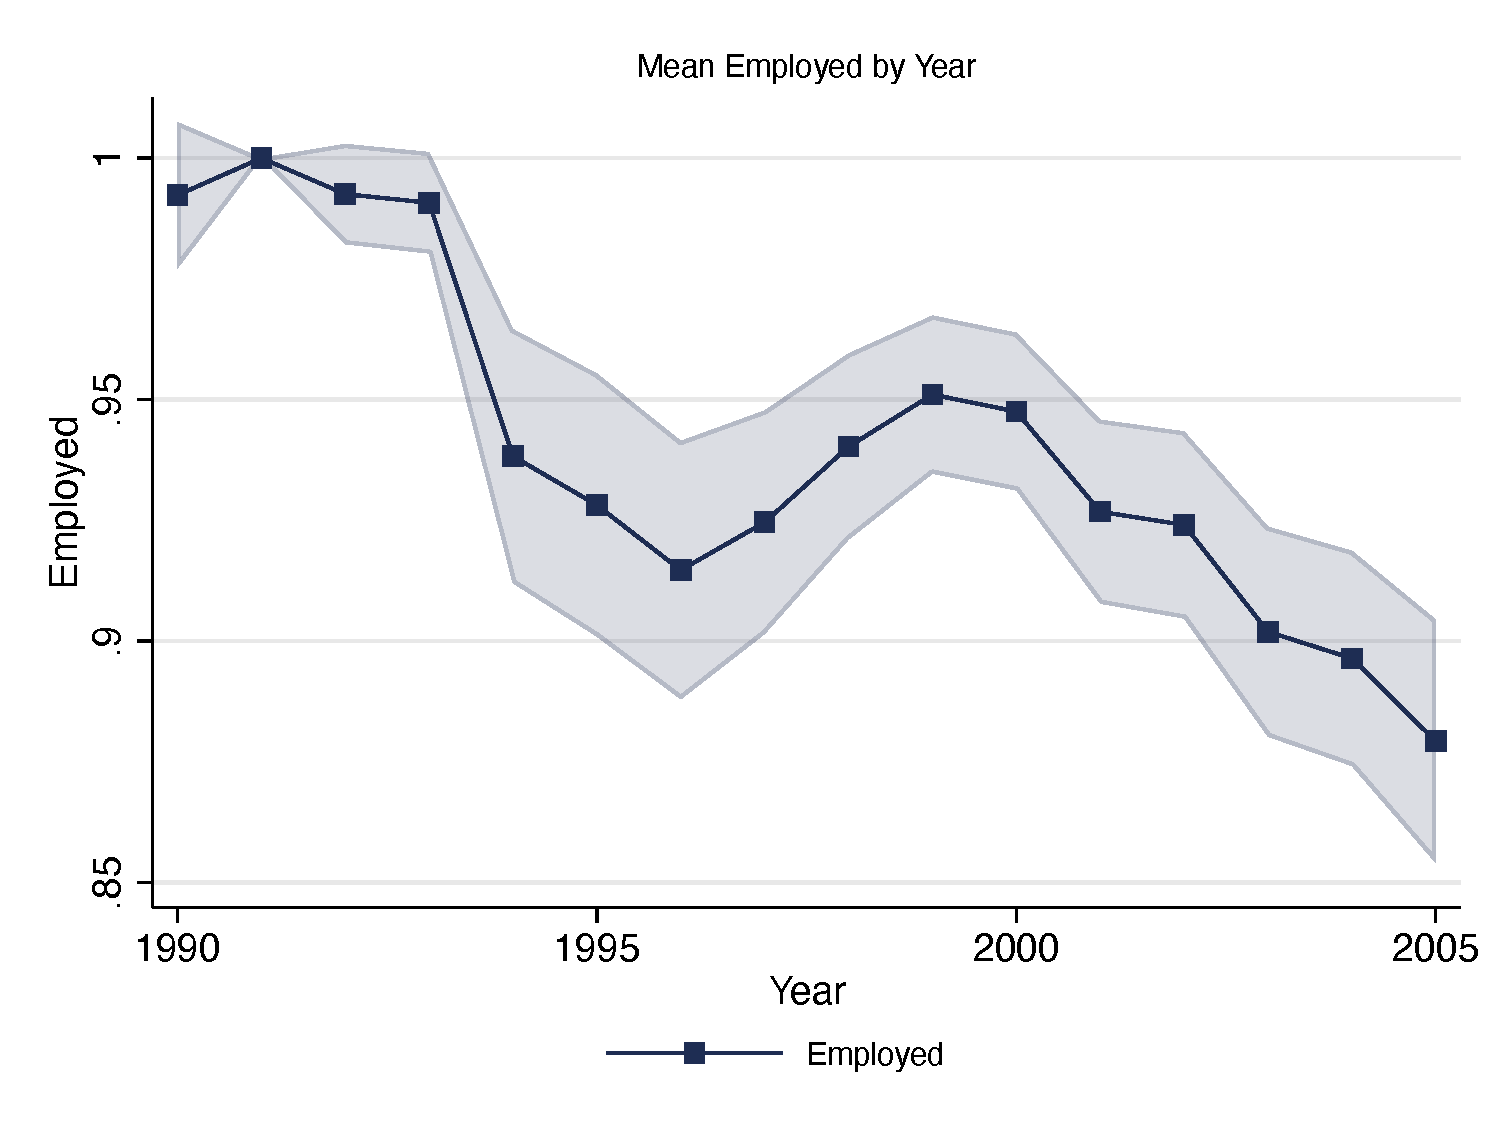
\includegraphics[width = .9\textwidth]{Consistency/employed_by_time.pdf} \\ 
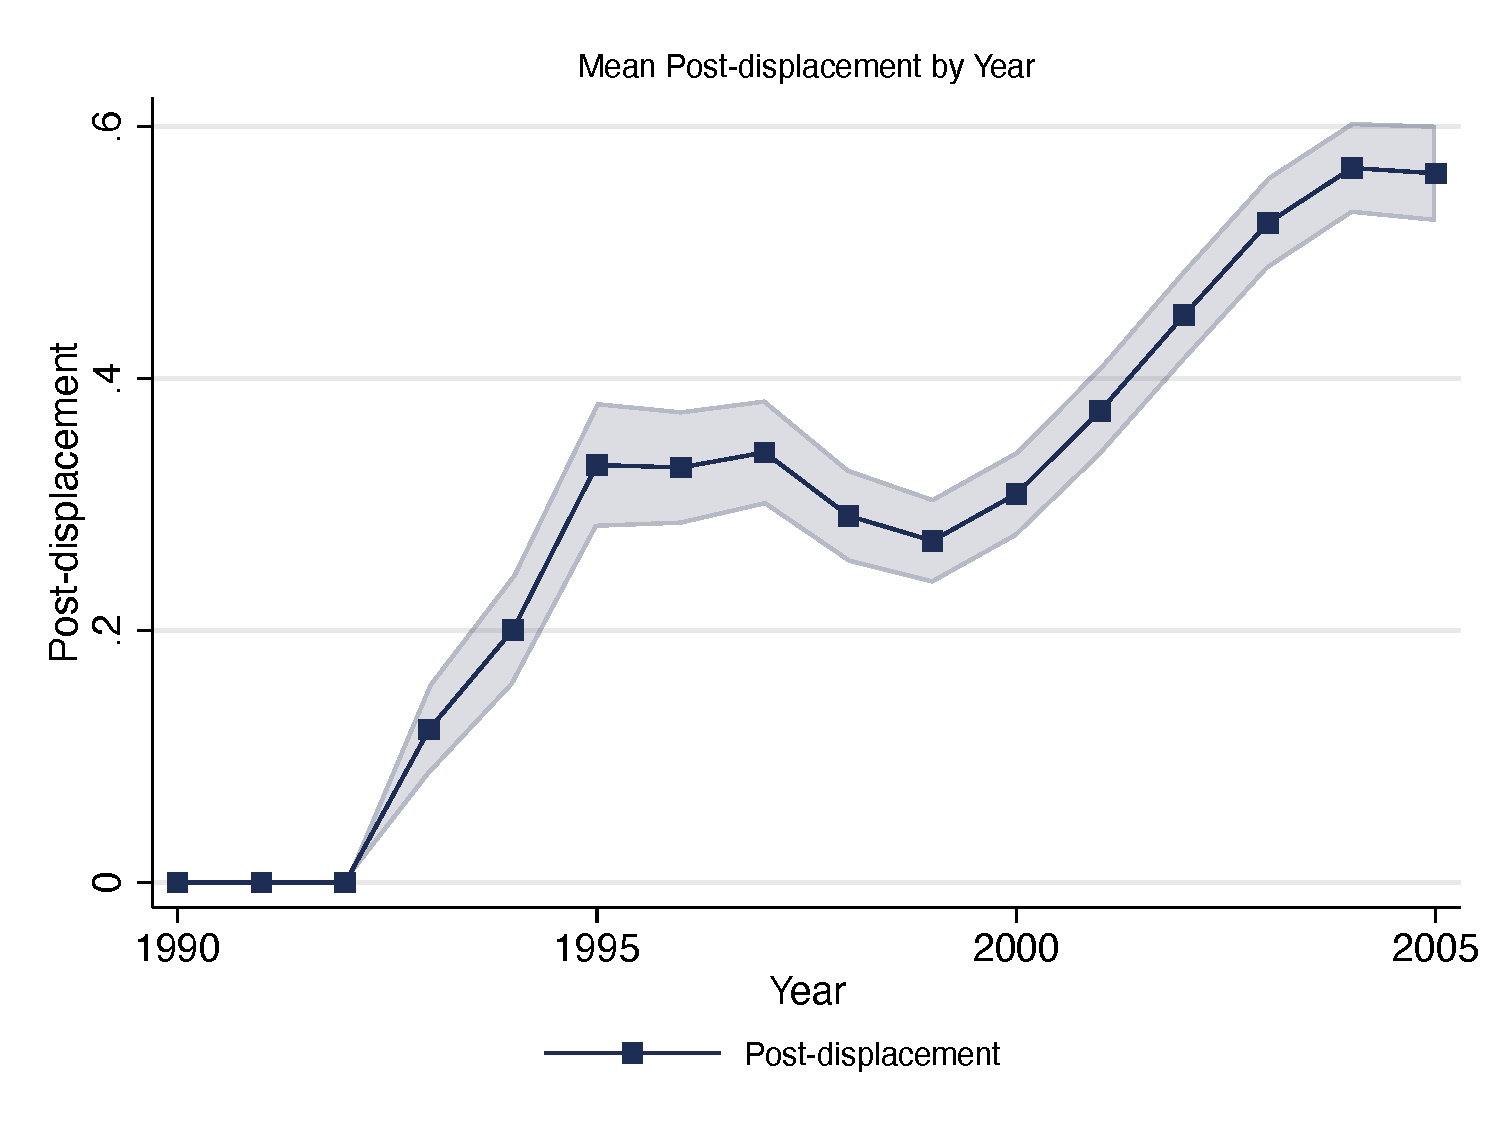
\includegraphics[width = .9\textwidth]{Consistency/displaced_by_time.pdf} \\ 
\section{Treatment and Control around Displacement Event}
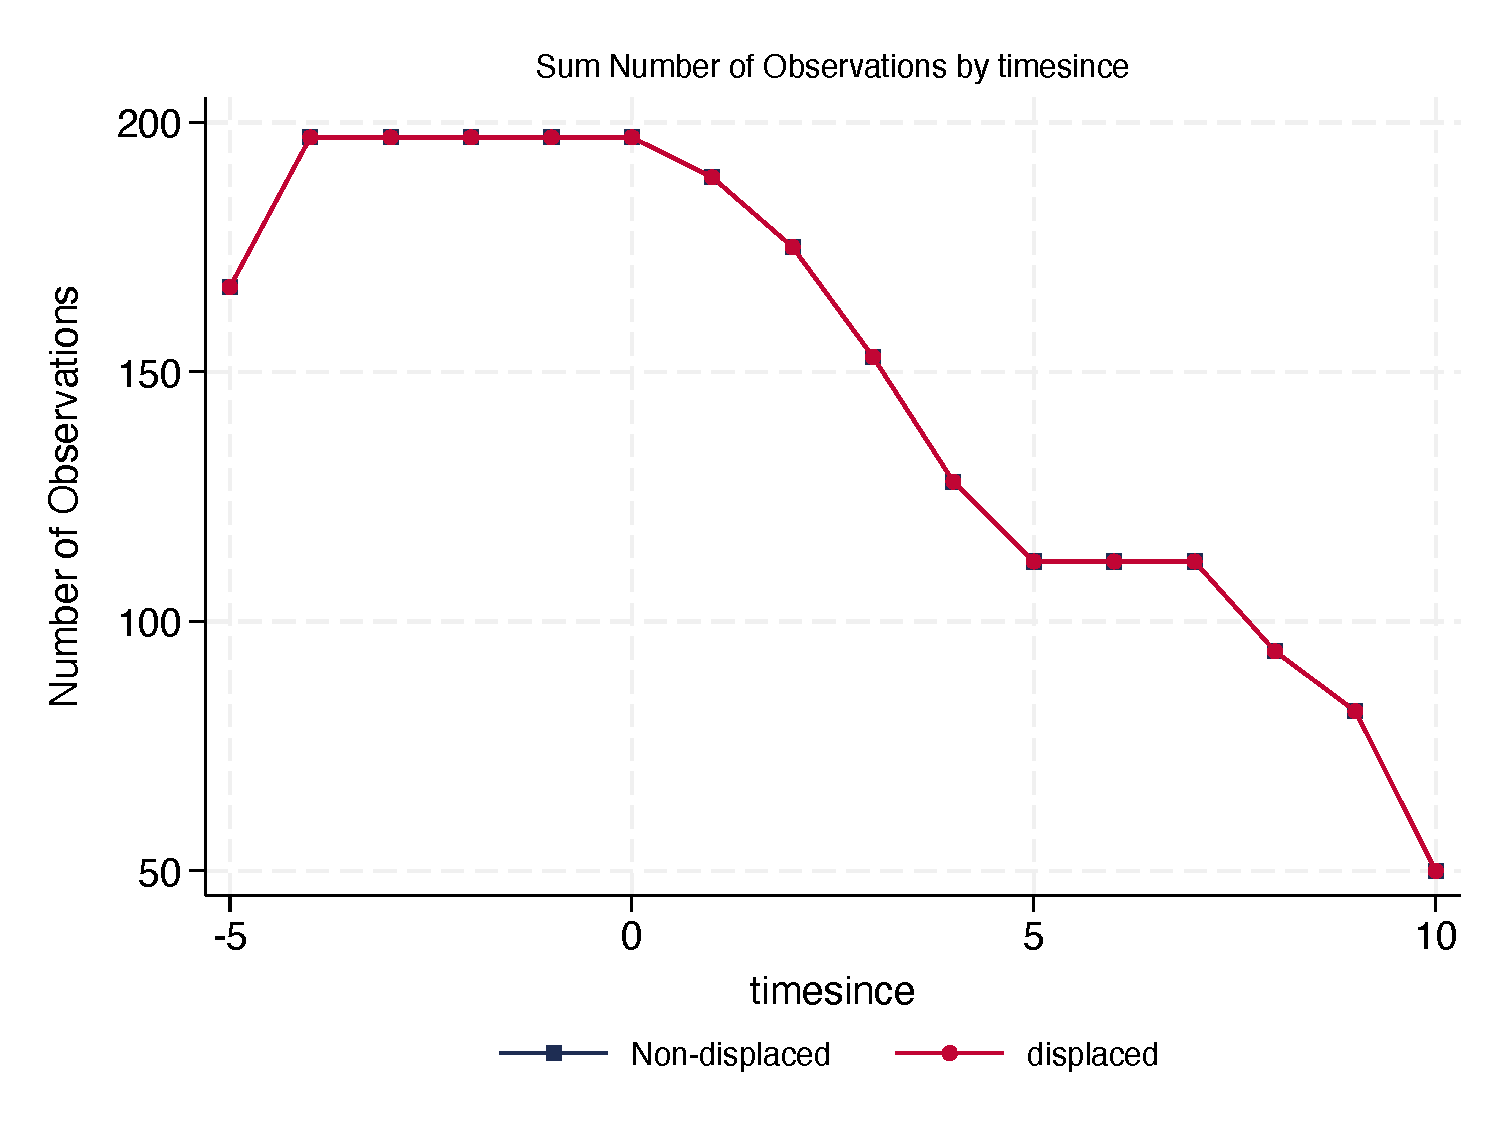
\includegraphics[width = .9\textwidth]{Disp_event_raw/counts_by_timesince.pdf} \\ 
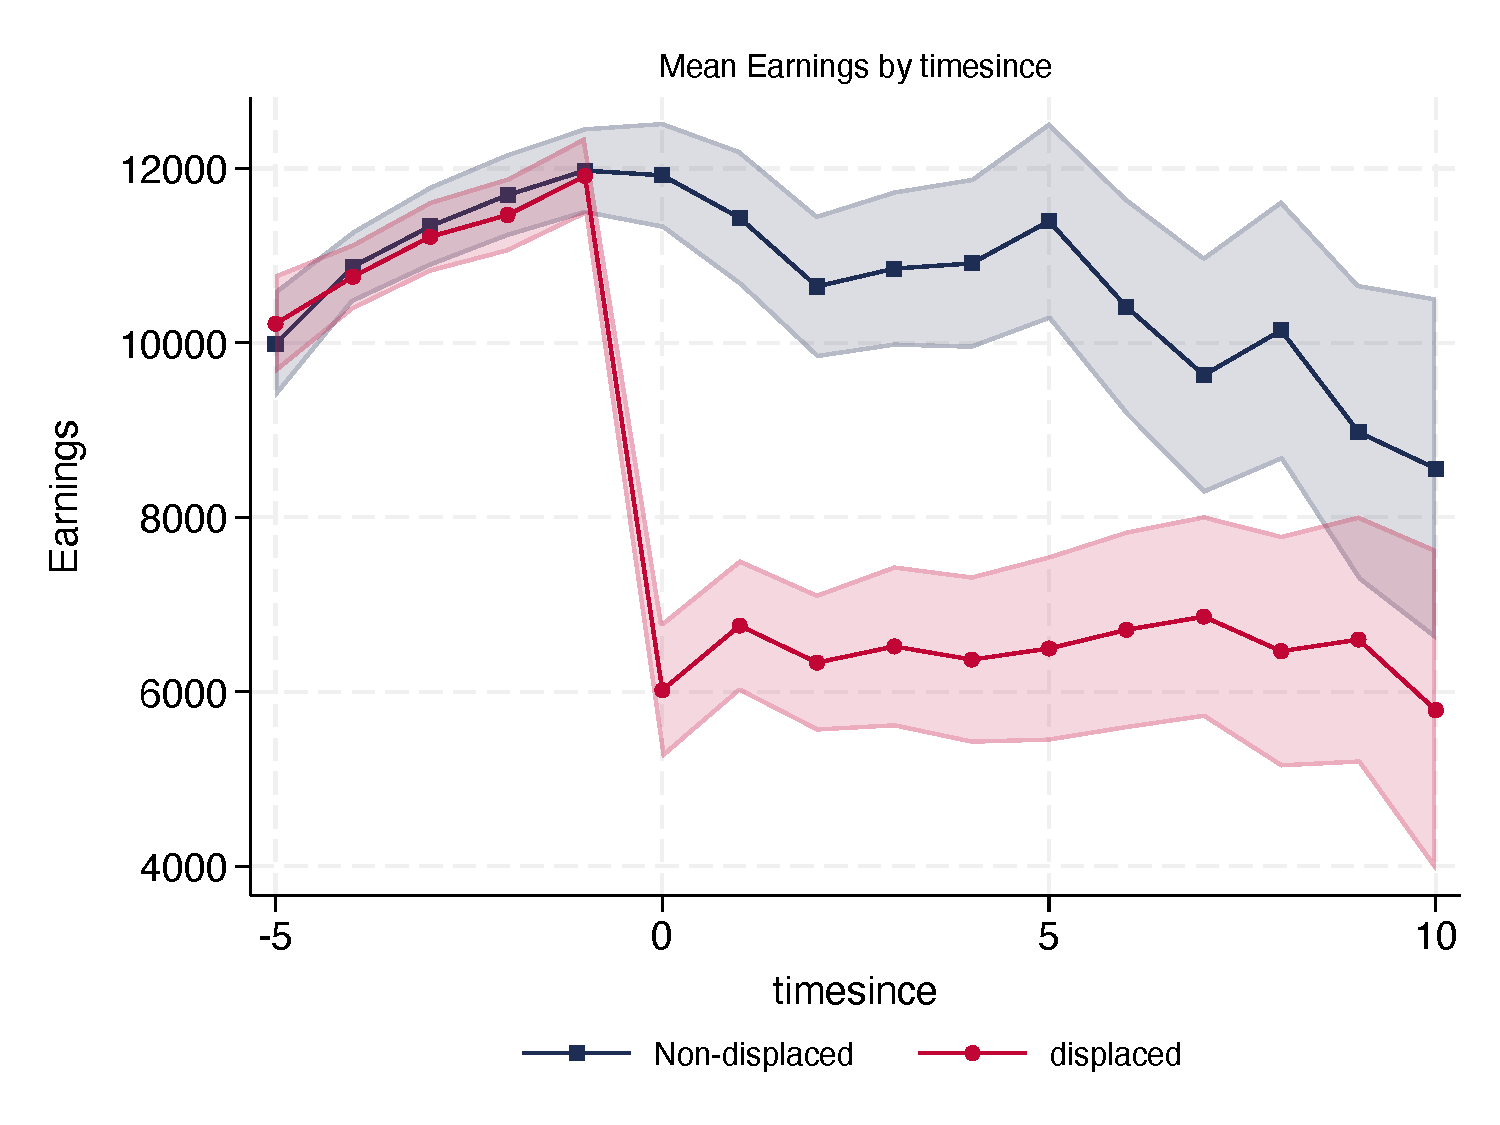
\includegraphics[width = .9\textwidth]{Disp_event_raw/logearn_by_timesince.pdf} \\ 

\end{document}
